\cleardoublepage\chapter{Introduction}
\minitoc\label{sec:introduction}\vspace{.5cm}

\section{Background and Motivation}

\sidenote{Research Context: Foo}
\todomid{write about the research context \gls{Foo}}\index{Foo}

\sidenote{Research Area: Bar}
\todomid{write about the research area and \Cref{fig:intro:a}}\index{Bar}

\begin{figure}[H]
    \centering
    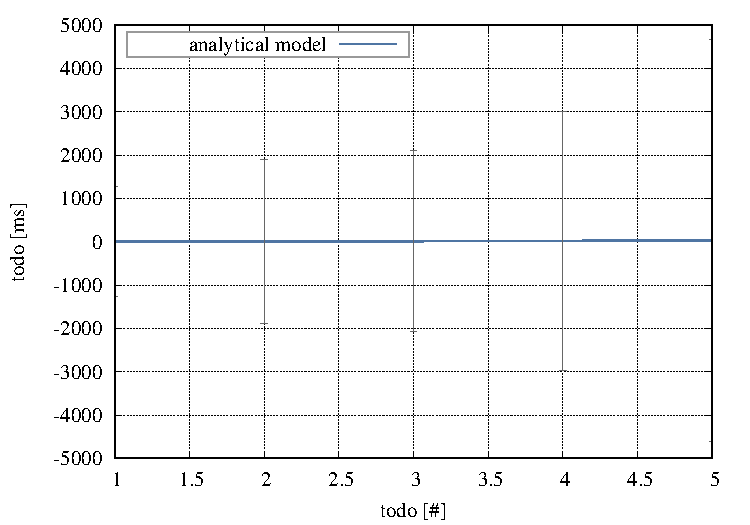
\includegraphics[width=.55\textwidth]{resources/images/example1}
    \caption{Example (based on~\cite{li2002design})}\label{fig:intro:a}
\end{figure}

\sidenote{Application Area: Foo Fooli}\index{Foo!Fooli}
\todomid{write about the application area~\cite{Heflin2004}}

\begin{figure}[H]
      \centering
      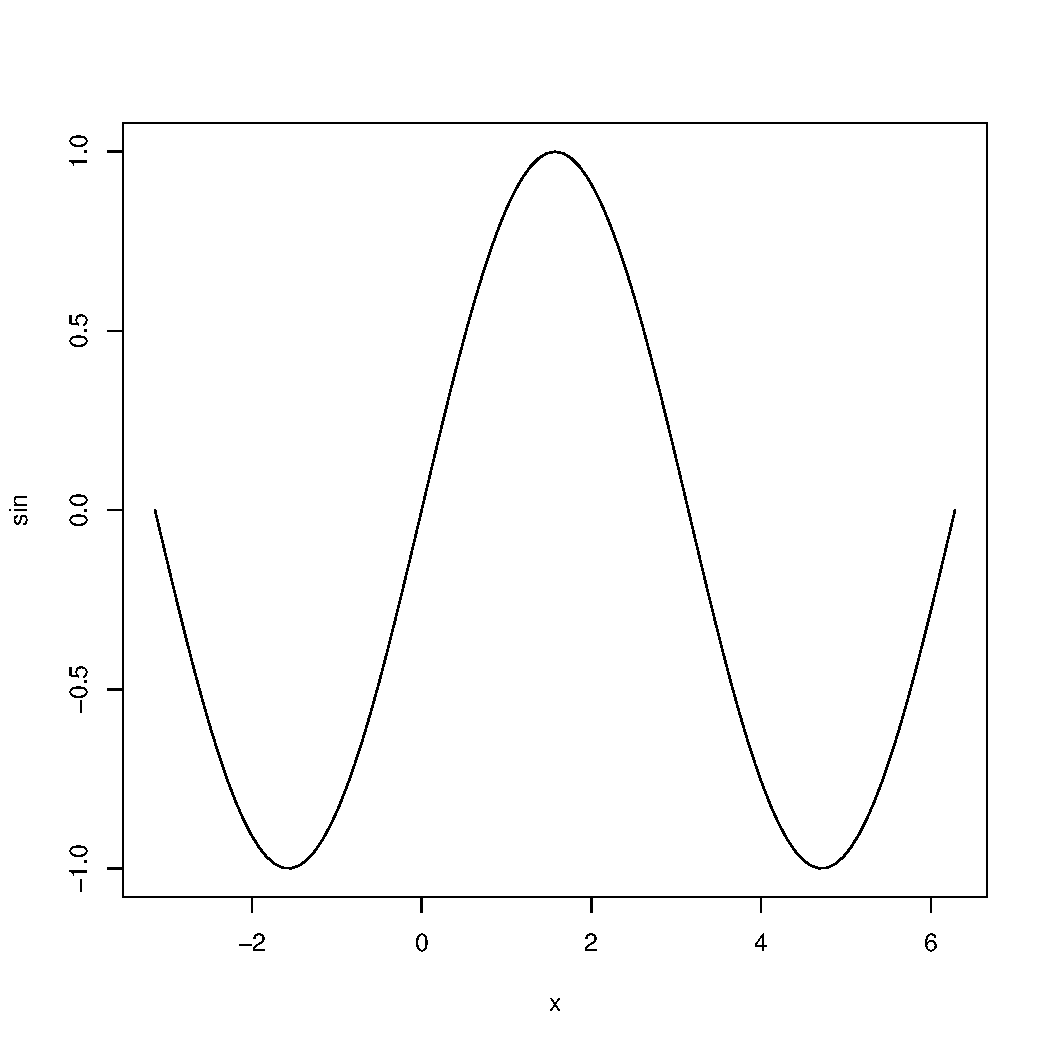
\includegraphics[width=.45\textwidth]{resources/images/example2}
      \caption{Another example~\cite{li2002design}}\label{fig:intro:b}
\end{figure}

\sidenote{Research Focus: Bar Barli}\index{Bar!Barli}
\todomid{write about the research focus and \Cref{fig:intro:b}}

\sidenote{Taxonomy}\index{Taxonomy}
\todomid{write about the taxonomy and \ac{ABAC}}

\begin{figure}[htbp]
      \centering
      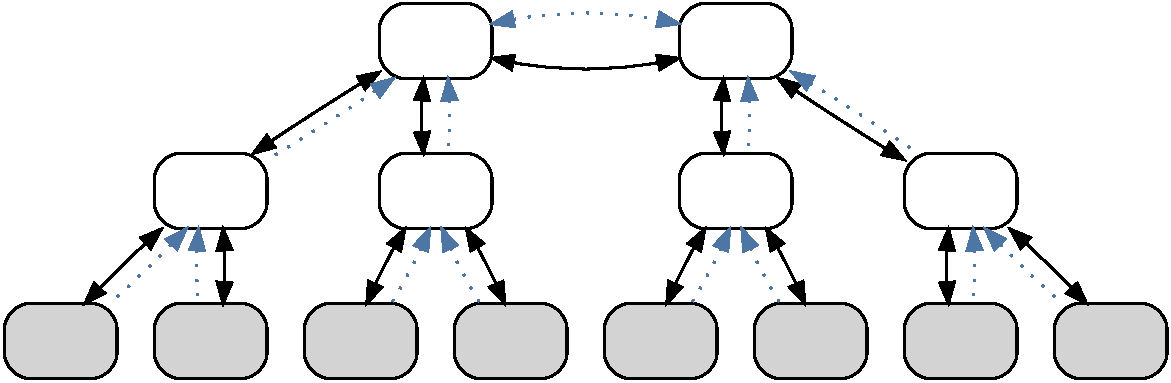
\includegraphics[width=.75\textwidth]{resources/images/example3}
      \caption{Taxonomy}
\end{figure}

\section{Problem Statement}\index{Requirements}

\sidenote{State of the Art}
\todomid{write about the State of the Art}

\sidenote{Issue:\\Example 1}
\todomid{write about the first issue}

\sidenote{Issue:\\Example 2}
\todomid{write about the second issue}

\sidenote{Synopsis}
\todomid{write about the synopsis of the issues and \Cref{fig:intro:c}}

\begin{figure}[htbp]
    \centering
    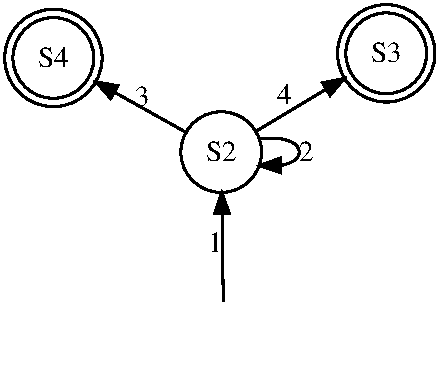
\includegraphics[width=.5\textwidth]{resources/images/job_lifecycle}
    \caption{Relationship between issues}\label{fig:intro:c}
\end{figure}

\section{Assumptions and Scope}

\sidenote{Research Assumptions}
\todomid{write about the research assumptions~\cite{li2002design}}

\sidenote{Research Scope}
\todomid{write about the research scope --- \Cref{fig:intro:a,fig:intro:b,fig:intro:c}}


\section{Objectives and Contributions}

\begin{figure}[htbp]
    \centering
    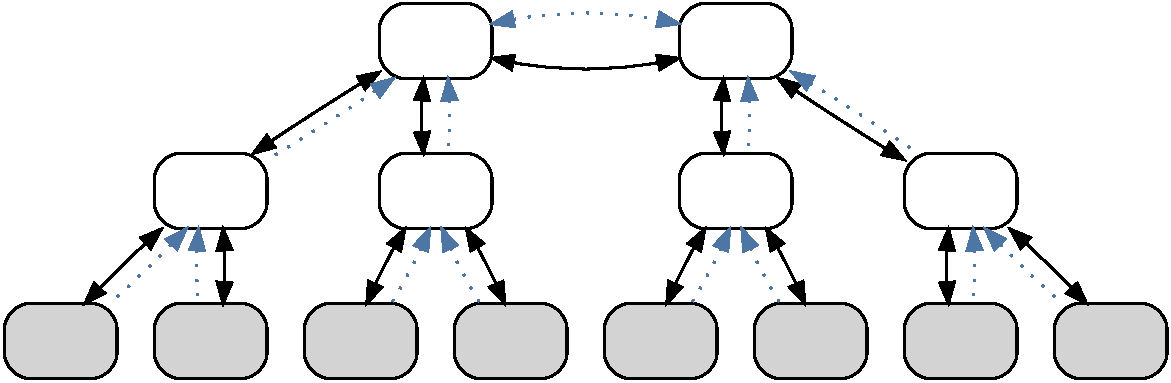
\includegraphics[width=.55\textwidth]{resources/images/example3}
    \caption{Structure of research}\label{fig:intro:struct}
\end{figure}

\sidenote{Research Objectives \& Contributions}
\todomid{write about the research objectives and \ac{DBpedia} and \Cref{fig:intro:struct}}

\section{Methodology and Outline}

\todomid{write about the research outline and \Cref{fig:intro:methodology}. Summarize \Cref{sec:introduction,sec:sota,sec:reqs,sec:contrib1,sec:contrib2,sec:contrib3,sec:eval,sec:summary}.}

\begin{sidewaysfigure}
    \centering
    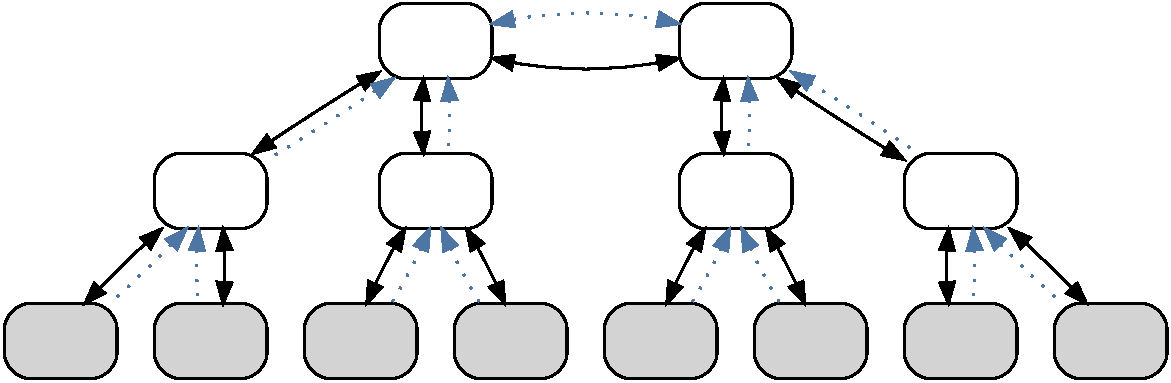
\includegraphics[width=.7\textwidth]{resources/images/example3}
    \caption{Workflow of the research and structure of the thesis}\label{fig:intro:methodology}
\end{sidewaysfigure}
